

\setchapterpreamble[c][.7\textwidth]{\itshape\color{gray}\small
    Der Begriff der Abbildung verallgemeinert den Funktionenbegriff aus der Schule. In diesem Vortrag werden grundlegende Begriffe, Sprech- und Schreibweisen im Umfeld von Abbildungen besprochen und durch Beispiele illustriert.
\vspace{24pt}}


\chapter{Abbildungen}


\section{Grundlegendes}


Ich werde das Kapitel sogleich mit einer Definition und einigen Allgemeinheiten beginnen. Falls dir das zu abstrakt anmutet, wirf schonmal einen Blick auf die Liste in \cref{bsp:abbildung}.


\begin{defin}[Abbildung] \label{def:abbildung} \index{Abbildung} \index{Funktion} \index{Definitionsbereich} \index{Wertebereich} \index{Graph (einer Abbildung)}
    Seien $X,Y$ zwei Mengen. Eine \textbf{Abbildung von $X$ nach $Y$} (oder auch \textbf{Funktion von $X$ nach $Y$}\footnote{Manche Leute bevorzugen das Wort „Abbildung“ im Umfeld abstrakter Mengen und das Wort „Funktion“ im Umfeld von $\R$. Ich werde aber beide Wörter völlig synonym verwenden.}) ist ein mathematisches Objekt, das \emph{jedem} Element von $X$ \emph{genau ein} Element von $Y$ zuordnet.

    Sind $f$ eine Abbildung von $X$ nach $Y$ und $x\in X$, so heißt das eindeutig bestimmte Element von $Y$, das $f$ dem Element $x$ zuordnet, der \textbf{Funktionswert von $f$ an der Stelle $x$} oder auch das \textbf{Bild von $x$ unter der Abbildung $f$} und wird notiert mit
    \begin{align*}
        f(x) && (\text{lies: „$f$ von $x$“})
    \end{align*}
    Ferner heißen
    \begin{itemize}
        \item $X$ der \textbf{Definitionsbereich} oder auch die \textbf{Quelle} von $f$ (englisch: ``domain'' oder ``source''),
        \item $Y$ der \textbf{Wertebereich} oder auch das \textbf{Ziel} von $f$ (englisch: ``codomain'' oder ``target''),
        \item die Menge $\{(x,y)\in X\times Y\mid y=f(x)\}$ der \textbf{Graph} von $f$.
    \end{itemize}
\end{defin}


\begin{axiom}[Gleichheit von Abbildungen] \label{abbgleich}
    Seien $X,Y$ zwei Mengen. Zwei Abbildungen $f,g$ von $X$ nach $Y$ stimmen genau dann überein, wenn sie an jeder Stelle denselben Funktionswert haben. Als Formel:
        \[ f=g \qquad\Leftrightarrow\qquad \forall x\in X:\ f(x)=g(x) \]
    Dementsprechend sind $f$ und $g$ voneinander verschieden, wenn es mindestens ein Element von $X$ gibt, an dem $f$ und $g$ verschiedene Funktionswerte annehmen.
    
    Zwei Abbildungen, die sich in ihrem Definitionsbereich oder ihrem Wertebereich unterscheiden, denkt man sich als „Objekte verschiedenen Typs“. Sie seien von vornherein voneinander verschieden.
\end{axiom}


\begin{nota}
    Seien $X,Y$ zwei Mengen.
    Anstelle von „$f$ ist eine Abbildung von $X$ nach $Y$“ schreiben wir kurz und bündig:
    \begin{align*}
        f:X \to Y \qquad & \text{oder auch}\qquad X\xrightarrow{f} Y && (\text{lies: „$f$ von $X$ nach $Y$“})
    \end{align*}
    Definitionsbereich, Wertebereich und Graph einer Abbildung $f$ werden manchmal notiert durch
        \[ \dom(f)\ , \qquad \codom(f) \qquad\text{und}\qquad \graph(f)\]
    Die Menge aller Abbildungen von $X$ nach $Y$ wird mit $\text{Abb}(X,Y)$ notiert:
        \[ \text{Abb}(X,Y) := \{ f \mid f\ \text{ist eine Abbildung von $X$ nach $Y$} \} \]
\end{nota}


\begin{nota}[Eine Abbildung über eine Zuordnungsvorschrift definieren] \label{def:zuordnung} \index{Zuordnungsvorschrift} \index{Abbildungsvorschrift} \index{Funktionsterm}
    Sei $t(a)$ ein Term in der Variablen $a$. Sind $X,Y$ zwei Mengen dergestalt, dass, setzt man für die Variable $a$ ein beliebiges Element aus $X$ ein, der Term $t$ stets ein Element von $Y$ ergibt, so heißt der Ausdruck
    \begin{align*}
        X \to Y \ &,\ x\mapsto t(x) && (\text{lies: „von $X$ nach $Y$, $x$ geht auf $t(x)$“})
    \end{align*}
    eine \textbf{Zuordnungsvorschrift} oder auch \textbf{Abbildungsvorschrift} von $X$ nach $Y$. Sie ist zu interpretieren als „Zuordnung“, die jedem Element $x\in X$ das Element $t(x)\in Y$, das durch Einsetzen des Objekts $x$ anstelle der Variablen $a$ zustandekommt, „zuordnet“. Der Term $t$ fungiert hier als sogenannter \textbf{Funktionsterm}.
    
    Jede solche Zuordnungsvorschrift definiert eine Abbildung $X\to Y$, deren Funktionswerte an Elementen $x\in X$ genau mit den Elementen $t(x)$ übereinstimmt. Möchte man diese Abbildung mit einer Variable bezeichnen, so schreibt man:
    \begin{align*}
        f : X\to Y \ & ,\ x\mapsto t(x) && (\text{lies: „$f$ von $X$ nach $Y$, $x$ geht auf $t(x)$“})
    \end{align*}
    Mit dieser Notation wird festgelegt, dass das Zeichen „$f$“ fortan diejenige Abbildung $X\to Y$ bezeichnen soll, die durch die Zuordnung $x\mapsto t(x)$ gegeben ist. Für jedes $x\in X$ gilt also $f(x)=t(x)$. Nach \cref{abbgleich} ist $f$ durch diese Eigenschaft eindeutig bestimmt.

    Im Ausdruck „$x\mapsto t(x)$“ fungiert das Zeichen „$x$“ als gebundene Variable im Sinne von \cref{gebundenevariable}.\footnote{Im für die Informatik relevanten \emph{Lambda-Kalkül} sagt man: „Die Variable $x$ wird durch $\lambda$-Abstraktion gebunden“, und schreibt „$\lambda x.t(x)$“ anstelle von $x\mapsto t(x)$.}
\end{nota}


\begin{bsp} \label{bsp:abbildung} \quad
    \begin{enumerate}
        \item Polynome ergeben Zuordnungen reeller Zahlen. Zum Beispiel:
        \begin{align*}
            f: \R \to \R \ & ,\ x  \mapsto x^2-1 \\
            g: \R \to \R \ & ,\  x  \mapsto 3x^2-2x+4
        \end{align*}
        Deren Definitions- und Wertebereich sind jeweils die Menge $\R$ der reellen Zahlen. Die Funktion $g$ ordnet jeder Zahl $x\in\R$ die Zahl $3x^2-2x+4$ zu, beispielsweise ist $g(4) = 3\cdot 16 - 2\cdot 4 + 4 = 44$.
        \begin{figure}[ht]
            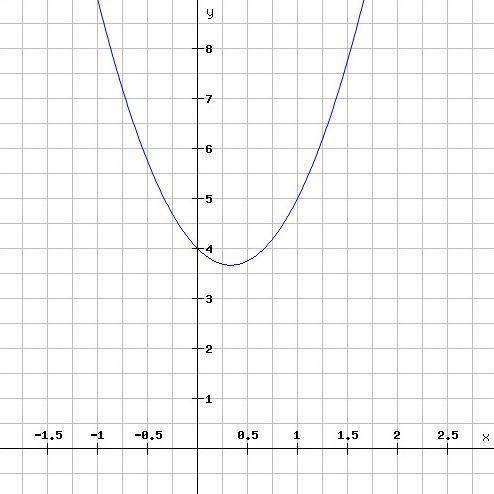
\includegraphics[width=9cm]{./_img/Polynom-Plot.jpeg}
            \centering \caption{Visualisierung des Graphen der Funktion $\R\to \R \ ,\ x\mapsto 3x^2-2x+4$}
        \end{figure}
        \item Seien $\mathtt{cat}$ die Menge aller Katzen und $\mathtt{colour}$ die Menge aller Farben. Wir haben eine Abbildung
            \[ f: \mathtt{cat} \to \mathtt{colour} \ ,\ C \mapsto (\text{Die Fellfarbe von $C$}) \]
        deren Definitionsbereich genau $\mathtt{cat}$ und deren Wertebereich genau $\mathtt{colour}$ ist. Für eine Katze $C$ ist $f(C)$ genau die Fellfarbe von $C$.
        \item Sei $X$ eine beliebige Menge. Die Abbildung
            \[ \{-\}: X \to \calP(X) \ ,\ x \mapsto \{x\} \]
        hat als Definitionsbereich $X$, als Wertebereich die Potenzmenge von $X$ und sie ordnet jedem Element $x \in X$ diejenige Einermenge zu, die nur aus $x$ besteht. 

        Der senkrechte Strich $-$ im Ausdruck „$\{-\}$“ meint einen Platzhalter, an dessen Stelle die Elemente des Definitionsbereichs „eingesetzt“ werden.
        \item Sei $\calA:=\{A\mid A\ \text{ist eine Aussage}\}$ die Menge aller mathematischen Aussagen. Die Junktoren $\land$ und $\neg$ ergeben Abbildungen
        \begin{align*}
            \calA\times \calA & \to \calA & \calA & \to \calA \\
            (A,B) & \mapsto A\land B & A& \mapsto \neg A
        \end{align*}
        d.h. im ersten Fall ordnen wir jedem Aussagenpaar $(A,B)$ die Konjunktion „$A$ und $B$“ zu und im zweiten Fall ordnen wir jeder Aussage ihre Negation zu. Ebenso liefern auch die anderen Junktoren $\lor,\to,\leftrightarrow$ jeweils Zuordnungen von Aussagen.
        \item Es bezeichne $\Set$ die Gesamtheit aller Mengen. Dann haben wir eine Abbildung
            \[ \Abb(-,-) : \Set \times \Set \to \Set \ ,\ (X,Y) \mapsto \Abb(X,Y) \]
        die jedem Mengenpaar $(X,Y)$ die Menge $\Abb(X,Y)$ aller Abbildungen $X\to Y$ zuordnet.
    \end{enumerate}
    Aus der Schule bist du es vielleicht gewohnt, dass der Graph einer Funktion eine Art „Kurve“ ist. Beachte, dass unsere allgemeine Graphendefinition deutlich abstrakter ist und der Graph einer Abbildung in der Regel keine „geometrische“ Bedeutung besitzt. Zumindest im Fall einer Abbildung $\R\to \R$ ist der Graph eine Teilmenge des $\R^2$, im Allgemeinen kann er aber alles andere als „kurvig“ aussehen.
\end{bsp}


\begin{vorschau}[* mengentheoretische Abbildungsdefinition]
    Die obige Definition einer Abbildung ist, ebenso wie die Mengendefinition \cref{def:menge}, rein axiomatisch. In der im 20. Jahrhundert vorherrschenden Praxis kann der Abbildungsbegriff formal präzise auf dem Mengen- und Elementbegriff aufgebaut werden: Eine Analyse ergibt, dass für zwei Abbildungen $f,g$ äquivalent sind:
    \begin{enumerate}[(i)]
        \item $f=g$.
        \item $\dom(f)=\dom(g)$, $\codom(f)=\codom(g)$ und $\graph(f)=\graph(g)$.
    \end{enumerate}
    \emph{Definiert} man nun eine Abbildung $f$ als ein Tripel $(X,G,Y)$ bestehend aus drei Mengen $X,G,Y$, wobei $G$ eine Teilmenge von $X\times Y$ mit der Eigenschaft, dass es für jedes $x\in X$ genau ein $y\in Y$ mit $(x,y)\in G$ gibt, sein soll, so wird daraufhin die Äquivalenz (i)$\leftrightarrow$(ii) zu einer beweisbaren Aussage, wohingegen sie in diesem Skript einfach als Axiom gegeben wurde.
    
    In der \href{https://en.wikipedia.org/wiki/Topos#Elementary_topoi_(topoi_in_logic)}{Topostheorie} wird dagegen umgekehrt verfahren: hier sind die „Abbildungen“ das fundamentale Konzept, das nicht definiert und nur durch Axiome beschrieben wird, worauf dann formal präzise die Begriffe von Element und Teilmenge aufgebaut werden.
    
    Weil ich keiner Herangehensweise den Vorzug geben will, werde ich es bei \cref{def:abbildung} belassen und nicht weiter auf eine formale Abbildungsdefinition eingehen.
\end{vorschau}


\begin{bem}[Beweisen, dass zwei Abbildungen gleich oder ungleich sind]
    Seien $X,Y$ zwei Mengen und $f,g:X\to Y$ zwei Abbildungen. Da das Gleichheitskriterium aus \cref{abbgleich} eine Allaussage ist (für \emph{jedes} $x\in X$ ist $f(x)=g(x)$), kann die Gleichheit $f=g$ nach \cref{allbeweis} dadurch bewiesen werden, dass ein „beliebiges“ Element von $X$ fixiert wird und dann bewiesen wird, dass dessen Funktionswerte unter $f$ und $g$ übereinstimmen.

    Bevor du überhaupt versuchst, die Gleichheit zweier Abbildungen zu beweisen, solltest du dich natürlich erstmal vergewissern, dass sie überhaupt denselben Definitionsbereich und denselben Wertebereich haben. Meistens ist das aber „offensichtlich“ und muss im Beweis nicht nochmal erwähnt werden.

    Um zu zeigen, dass zwei Abbildungen verschieden sind, genügt es nach \cref{gegenbeispiel}, ein Gegenbeispiel anzugeben, d.h. in diesem Fall, ein Element $x\in X$ zu finden, für das $f(x)\neq g(x)$.
\end{bem}


\begin{bsp} \label{bsp:abbgleich} \quad
    \begin{enumerate}
        \item Betrachten wir die Abbildungen: 
        \begin{align*}
            f: \R \to \R\ &,\ x \mapsto x^2 \\
            g: \R \to \R\ &,\ x \mapsto 2x+1
        \end{align*}
        So ist $f \neq g$, denn es ist $f(1)=1$ und $g(1)=3$.
        \item Betrachten wir dagegen die Abbildungen
        \begin{align*}
            \alpha: \R \to \R\ &,\ x \mapsto (x+1)\cdot (x-1) \\
            \beta: \R \to \R\ &,\ x \mapsto  x^2-1
        \end{align*}
        so gilt für jede beliebige reelle Zahl $x\in \R$, dass
            \[ \alpha(x) = (x+1)(x-1) = x^2-1 = \beta(x) \]
        Demnach ist $\alpha=\beta$.
    \end{enumerate}
\end{bsp}


\begin{bem}[Zuordnungsvorschriften vs. Abbildungen] \label{zuordvsabb}
    Jede Zuordnungsvorschrift kann zur Definition einer Abbildung verwendet werden. Beachte, dass Zuordnungsvorschriften und Abbildungen nicht ganz dasselbe sind. Eine Zuordnungsvorschrift ist ein sprachliches Gebilde, eine konkrete Vorschrift, wie Gegenständen vom Typ $X$ Gegenstände vom Typ $Y$ zuzuordnen seien, wohingegen der Abbildungsbegriff eine mathematische Abstraktion darstellt. Das Verhältnis zwischen Termen und Abbildungen ist, genau wie das zwischen Eigenschaften und Mengen (vgl. \cref{mengenvseig}), ein Aspekt der Dualität zwischen Syntax und Semantik (siehe \cref{syntaxvssemantik}).
    \begin{itemize}
        \item Dieselbe Abbildung kann durch verschiedene Zuordnungsvorschriften zustandekommen. Beispielsweise sind
        \begin{align*}
            \R \to \R \ &,\ x\mapsto x^2-1 \\
            \R \to \R \ &,\ x\mapsto (x+1)(x-1)
        \end{align*}
        zwei verschiedene Zuordnungsvorschriften, die aber nach \cref{bsp:abbgleich} dieselbe Abbildung darstellen.
        \item Nicht jede Abbildung muss durch eine einfache Zuordnungsvorschrift definierbar sein. Abbildungsvorschriften können beliebig kompliziert sein und manche Abbildungen sind so chaotisch, dass sie gar keiner Abbildungsvorschrift gehorchen. Beispielsweise beweist man in der Berechenbarkeitstheorie, dass es Abbildungen $\N \to \{0,1\}$ (also Abfolgen von Nullen und Einsen) geben muss, die nicht Turing-berechenbar\footnote{\href{https://de.wikipedia.org/wiki/Alan_Turing}{Alan Turing (1912-1954)}} sind, d.h. die so chaotisch sind, dass es keinen konventionellen Algorithmus gibt, der nacheinander alle Folgenglieder auflistet.
        \item Definitions- und Wertebereich sind grundlegende Bestandteile einer Abbildung. Beispielsweise kann der Ausdruck
            \[ x\mapsto x^2 \]
        in verschiedenfacher Weise als Zuordnungsvorschrift interpretiert werden, z.B. als Zuordnung $\R\to \R$, $\Z\to \N_0$ oder $\C\to \C$. Die drei Abbildungen
        \begin{align*}
            \R \to \R \ & ,\ x\mapsto x^2 \\
            \Z \to \N_0 \ & ,\ x\mapsto x^2 \\
            \C \to \C \ &,\ x\mapsto x^2 
        \end{align*}
        sind aber allesamt voneinander verschieden, da sie verschiedene Definitions- und Wertebereiche haben. Siehe auch \cref{bsp:injsur}.
    \end{itemize}
\end{bem}


\begin{bem}[Funktionen „in mehreren Variablen“]
    Nach unserer Abbildungsdefinition kann in eine Abbildung $f:X\to Y$ genau ein Element $x$ aus $X$ „eingesetzt“ werden, um genau ein Element $f(x)$ von $Y$ zu erhalten. Dies erweckt vielleicht den Anschein, dass unsere Abbildungsdefinition nicht in der Lage wäre, „Funktionen in mehreren Veränderlichen“ wie zum Beispiel
        \[ x,y \quad\mapsto\quad 2xy + xy^2 \]
    zu modellieren. -- Sie ist es aber, und der Trick besteht in der Verwendung des kartesischen Produkts als Definitionsbereich. Beispielsweise haben wir eine Abbildung
        \[ \R \times \R \to \R \ ,\ (x,y) \mapsto 2xy +xy^2 \]
    Verwenden wir noch allgemeinere Produkte $\prod_{i\in I} M_i$ als Definitionsbereich, können wir auch „Funktionen in unendlich vielen Variablen“ definieren.
\end{bem}





\section{Verketten von Abbildungen}


\begin{defin}[Verketten von Abbildungen]\label{def:verkettung} \index{Verkettung von Abbildungen}
    Seien $X,Y,Z$ drei Mengen und $X\xrightarrow{f} Y$, $Y \xrightarrow{g} Z$ zwei Abbildungen. Mit
    \begin{align*}
        g\circ f && (\text{lies: „$g$ nach $f$“ oder „$g$ kringel $f$“})
    \end{align*}
    wird diejenige Abbildung $X\to Z$ bezeichnet, die gegeben ist durch die Zuordnungsvorschrift
    \begin{align*}
        X \to Z \ ,\ x \mapsto g(f(x))
    \end{align*}
    Die Abbildung $g\circ f$ heißt die \textbf{Verkettung}, \textbf{Komposition} oder \textbf{Hintereinanderausführung} von $f$ und $g$.
    
    Insgesamt erhalten wir eine Abbildung
        \[ \circ : \Abb(Y,Z)\times \Abb(X,Y) \to \Abb(X,Z) \ ,\ (g,f) \mapsto g\circ f\]
\end{defin}


\begin{bem} \quad
    \begin{itemize}
        \item Beachte, dass in der Notation „$g\circ f$“ diejenige Abbildung, die „zuerst“ ausgeführt wird, an rechter Stelle steht. Für ein Element $x \in X$ berechnet man $(g\circ f)(x)$, indem man zuerst $f(x)$ ausrechnet und darauf nun die Abbildung $g$ anwendet.
        \item Sind zwei Abbildungen durch Funktionsterme gegeben, so erhält man ihre Verkettung durch Einsetzen des einen Terms in den anderen im Sinne von \cref{def:substitution}, siehe dazu die nachfolgenden Beispiele. Dies ist ein Aspekt der Dualität zwischen Syntax und Semantik (siehe \cref{syntaxvssemantik}).
    \end{itemize}
\end{bem}


\begin{bsp}
    Es seien $S:= \{ \text{Schauspieler in Filmen}\}$ die Menge aller Filmdarsteller und $F:=\{\text{Filme}\}$ die Menge aller Filme. Wir haben Abbildungen
    \begin{align*}
        f : S \to F \ & ,\ s\mapsto (\text{Der erste Film, in dem $s$ mitgespielt hatte}) \\
        g : F \to \N \ & ,\ x \mapsto (\text{Das Jahr, in dem die Dreharbeiten an $x$ begannen})
    \end{align*}
    Dann ist die Verkettung $g\circ f$ diejenige Abbildung $S\to \N$, die jedem Schauspieler das Jahr zuordnet, in dem der erste Film, bei dem er mitgespielt hat, gedreht wurde.
\end{bsp}


\begin{bsp} \label{bsp:verkettung}
    Betrachte die Abbildungen
    \begin{align*}
        f : \R \to \R \ &,\ x\mapsto x^2 \\
        g : \R \to \R \ &,\ x \mapsto x-1
    \end{align*}
    Dann gilt für $x\in \R$:\footnote{vgl. \cref{bsp:substitution}}
    \begin{align*}
        (g\circ f)(x) & = g(f(x)) = g(x^2) = x^2-1 \\
        (f\circ g)(x) & = f(g(x)) = f(x-1) = (x-1)^2
    \end{align*}
    Wegen $(g\circ f)(4)\neq (f\circ g)(4)$ ist $g\circ f\neq f\circ g$.
\end{bsp}


\begin{vorschau}[Integration durch Substitution]
    Die Technik, einer Abbildung $g$ eine Abbildung $f$ „vorzuschalten“, kennst du vielleicht schon aus der Schule als „Variablensubstitution“. Bei der sogenannten „Integration durch Substitution“ spielt dies eine maßgebliche Rolle. Sind $f,g:\R\to \R$ zwei hinreichend „glatte“ Funktionen und $a,b\in \R$, so besagt die Substitutionsregel, dass
        \[ \int_{f(a)}^{f(b)} g = \int_a^b (g\circ f) \cdot f' \]
    Falls du diese Methode nicht kennst, ist das nicht schlimm. Sie wird üblicherweise in der Ana1- oder Ana2-Vorlesung thematisiert.
\end{vorschau}


\begin{satz}[Verketten von Abbildungen ist assoziativ] \label{abbassoziativ}
    Seien $A,B,C,D$ vier beliebige Mengen und
    \[\begin{tikzcd}
        A \ar[r, "f"] & B \ar[r, "g"] & C \ar[r, "h"] & D
    \end{tikzcd}\]
    drei Abbildungen. Dann gilt:
        \[ h\circ (g\circ f) = (h\circ g)\circ f\]
\end{satz}


\begin{bew}
    Für jedes $a \in A$ ist
    \begin{align*}
        \bigl(h \circ (g \circ f)\bigr)(a) & =h\bigl((g \circ f)(a)\bigr)\\
        & =h\bigl(g(f(a))\bigr) \\
        & =\bigl(h \circ g\bigr) \bigl(f(a)\bigr) \\
        & = \bigl((h \circ g) \circ f\bigr) (a)	
    \end{align*}
    Da das Element $a\in A$ beliebig gewählt war, folgt $h\circ (g\circ f) = (h\circ g)\circ f$. \qed
\end{bew}


\begin{bem}[Klammern sparen] \label{abbklammerfrei}
    Aufgrund von \cref{abbassoziativ} wird in dessen Situation einfach
        \[ h\circ g\circ f \]
    geschrieben, da es egal ist, ob erst $g$ mit $f$ verkettet wird und dann $h$ mit $g\circ f$ -- oder ob erst $h$ mit $g$ verkettet wird und dann $f$ mit $h\circ g$. Mit fortgeschrittenen Techniken lässt sich zeigen, dass es auch bei Verkettungen von mehr als drei Abbildungen egal ist, wie man Klammern setzt. Daher werden Klammerungen meist ganz weggelassen.\footnote{vgl. dazu auch \cref{klammerfrei}} Sind etwa $A,B,C,D,E,F$ sechs Mengen und sind Abbildungen
    \[\begin{tikzcd}
        A \ar[r, "a"] & B \ar[r, "b"] & C \ar[r, "c"] & D \ar[r, "d"] & E \ar[r, "e"] & F
    \end{tikzcd}\]
    gegeben, so wird mit
        \[ e\circ d\circ c\circ b\circ a \]
    diejenige Abbildung notiert, die durch Verkettung dieser fünf Abbildungen entsteht, die sich also dadurch zusammensetzt, dass erst $a$ durchlaufen wird, dann $b$, dann $c$, dann $d$ und zuletzt $e$.
\end{bem}





\section{Identität und Inklusion}


Sei $X$ eine beliebige Menge. Gibt es überhaupt eine Abbildung $X\to X$? Solange wir keine Informationen über die Elemente von $X$ haben, können wir ja schwerlich eine besondere Abbildungsvorschrift angeben. Dennoch gibt es stets eine Abbildung $X\to X$, deren Zuordnungsvorschrift so simpel ist, dass man sie schon wieder übersehen könnte:


\begin{defin}[Identitätsabbildung] \index{Identität}
    Sei $X$ eine Menge. Die Abbildung
    \begin{align*}
        \id_X: X \to X \ ,\ x \mapsto x
    \end{align*}
    heißt die \textbf{Identität auf $X$}.
\end{defin}


\begin{bem}
    Die Identität auf der Menge $X$ bildet jedes Element auf sich selbst ab und „tut gar nichts“. Die Identität auf $\R$ kennst du auch schon aus der Schule: die Polynomfunktion „$f(x)=x$“ ist genau die Identitätsabbildung $\id_\R$ auf der Menge der reellen Zahlen.
\end{bem}


\noindent Der nächste Satz zeigt, dass sich die Identität hinsichtlich der Verkettung von Abbildungen verhält, wie die $0$ bei der Addition oder die $1$ bei der Multiplikation, vgl. \cref{def:neutrales}.


\begin{satz}[Neutralität der Identität] \label{idneutral}
    Seien $X,Y$ zwei beliebige Mengen und $X\xrightarrow{f} Y$ eine Abbildung. Dann gilt:
    \begin{align*}
        f\circ \id_X & = f \\
        \id_Y \circ f & = f
    \end{align*}
\end{satz}


\begin{bew}
    Ist $x \in X$ ein beliebiges Element, so gilt
    \begin{align*}
        (f\circ \id_X)(x) & = f(\id_X(x)) \\
        & =f(x) && (\text{per Definition von $\id_X$}) \\
        (\id_Y \circ f)(x) & =\id_Y(f(x)) \\
        & = f(x)&& (\text{per Definition von $\id_Y$})
    \end{align*}
    Da das Element $x\in X$ beliebig gewählt war, folgt $f\circ \id_X=f$ und $\id_Y\circ f=f$. \qed
\end{bew}


\begin{vorschau}[* Die Kategorie der Mengen] \label{kategorien}
    Die Sätze \cref{idneutral} und \cref{abbassoziativ} lassen sich auch so zusammenfassen, dass Mengen und Abbildungen die Struktur einer sogenannten \href{https://ncatlab.org/nlab/show/category}{Kategorie} bilden. Die Sprache der Kategorien ist von fundamentaler Bedeutung für die gesamte Mathematik und du wirst, falls du in die reine Mathematik gehst, in deinem Studium noch haufenweise weitere Kategorien kennenlernen. Zum Beispiel:
    \begin{longtable}{lccr}
    Fachgebiet & \phantom{Platzhalter} & Kürzel & \phantom{Platzhalterhalter} Kategorie \\
    \midrule
    Grundlagen && $\Set$ & Mengen \\ 
    && $\Pos$ & Geordnete Mengen \\[0.5em]
    Lineare Algebra && ${}_K\mathsf{Vec}$ & $K$-Vektorräume \\
    && ${}_R\mathsf{Mod}$ & $R$-Moduln \\
    && ${}_R\mathsf{Mat}$ & Matrizen über $R$ \\[0.5em]
    Analysis && $\mathsf{Top}$ & Topologische Räume \\
    && $\mathsf{Met}$ & Metrische Räume \\
    && $\mathsf{Man}$ & Mannigfaltigkeiten \\
    && $\sigma\textsf{-Alg}$ & Sigma-Algebren \\[0.5em]
    Algebra && $\Mon$ & Monoide \\
    && $\Grp$ & Gruppen \\
    && ${}_G\Set$ & $G$-Mengen \\
    && $\mathsf{Ring}$ & Ringe \\
    && ${}_R\mathsf{Alg}$ & $R$-Algebren \\[0.5em]
    Funktionalanalysis && $\mathsf{Unif}$ & Uniforme Räume \\
    && $\mathsf{Ban}$ & Banachräume \\
    && $\mathsf{Hilb}$ & Hilberträume \\[0.5em]
    Fortgeschrittene Vorlesungen && $\mathsf{Cat}$ & Kategorien \\
    && $\Sh(\calC)$ & Garben auf $\calC$ \\
    && $\Delta$ & Simplexkategorie \\
    && $\mathsf{sSet}$ & Simpliziale Mengen \\
    && $\Ch(\calA)$ & Komplexe in $\calA$ \\
    && $\mathsf{Sch}$ & Schemata \\
    \end{longtable}
\end{vorschau}


\begin{defin}[Inklusionsabbildung] \label{def:inklusion} \index{Inklusion (einer Teilmenge)}
    Seien $X$ eine Menge und $U\subseteq X$ eine Teilmenge. Die \textbf{Inklusionsabbildung} (oder auch kurz: \textbf{Inklusion}) von $U$ in $X$ ist die Abbildung
    \begin{align*}
        U \to X \ ,\ x \mapsto x
    \end{align*}
    meist notiert mit dem griechischen Buchstaben $\iota$ (Iota) und einem Pfeil „$\hookrightarrow$“ mit Haken:
        \[ \iota_U : U \hookrightarrow X \]
    Gelegentlich spricht man auch von der \emph{natürlichen Inklusion} oder der \emph{kanonischen Inklusion}.
\end{defin}


\begin{bem}
    Die natürliche Inklusion ordnet einem Element aus $U$ genau das gleiche Element in $X$ zu. Genauso wie bei der Identitätsabbildung werden auch von der Inklusion keine Elemente verändert. Allerdings bewirkt die Inklusion eine „Kontextverschiebung“. Ist $x\in U$ irgendein Objekt, von dem betont ist, dass es ein Element von $U$ ist, so ist $\iota(x)$ nachwievor dasselbe Objekt, jetzt aber betont als Element von $X$.
    
    Der „behakte Pfeil $\hookrightarrow$“ ist schlicht eine Variante zum gewöhnlichen Abbildungspfeil, die bei Abbildungen auftritt, die sich ähnlich wie die natürliche Inklusion verhalten. Er wird verwendet, um den „Inklusionscharakter“ einer Abbildung hervorzuheben. 
\end{bem}


\begin{bsp}
    Man hat eine Inklusionsabbildung $\iota : \Z \to \Q$, die jede ganze Zahl auf sich selbst, nun aufgefasst als rationale Zahl, abbildet.
\end{bsp}


\begin{bem}[„Kanonizizät“ der natürlichen Inklusion]
    Seien $X$ eine beliebige Menge und $U\subseteq X$ eine Teilmenge. Notiert man ohne weitere Spezifikation einen Pfeil „$U\hookrightarrow X$“, so ist damit in der Regel die natürliche Inklusion gemeint. Denn welche „selbstverständliche“ Abbildung sollte es, sofern dir keine weiteren Informationen über $X$ und $U$ bekannt sind, außer dass eben $U$ eine Teilmenge von $X$ ist, sonst noch von $U$ nach $X$ geben?
    
    Darin besteht das „Natürliche“ an der natürlichen Inklusion: dass man mit ihr völlig unabhängig von der konkreten Gestalt von $X$ und der Teilmenge $U$ stets eine konkrete Abbildung $U\to X$ zur Hand hat.
\end{bem}


\begin{defin}[* Leere Abbildung] \index{Leere Abbildung}
    Sei $X$ eine beliebige Menge. Dann gibt es genau eine Abbildung $\emptyset\to X$, die sogenannte \textbf{leere Abbildung}. Es handelt sich genau um die natürliche Inklusion der Teilmenge $\emptyset\subseteq X$, vgl. \cref{leeremengeimmerdrin}.
\end{defin}





\section{Bilder und Urbilder von Teilmengen}


\begin{defin}[Bild und Urbild von Teilmengen] \label{def:bildmenge} \index{Faser} \index{Bild} \index{Urbild}
    Seien $X,Y$ Mengen und $X \xrightarrow{f} Y$ eine Abbildung.
    \begin{itemize}
        \item Für ein Element $y\in Y$ heißt die Menge
            \[ f^{-1}(y) := \{ x\in X \mid f(x)=y \} \]
        die \textbf{Faser von $y$} (unter der Abbildung $f$). Man spricht auch vom \textbf{Urbild von $y$}. Die Elemente von $f^{-1}(y)$ werden ebenfalls \textbf{Urbilder von $y$} genannt.
        \item Die Menge
            \[ \im(f) := \{y\in Y\mid \exists x\in X:\ f(x)=y  \} \]
        heißt das \textbf{Bild von $f$} (englisch: ``image'').
        \item Für eine Teilmenge $B\subseteq Y$ heißt
            \[ f^{-1}(B) := \{ x \in X \mid f(x)\in B \} \]
        die \textbf{Urbildmenge von $B$} oder schlicht das \textbf{Urbild} von $B$ unter $f$.
        \item Für eine Teilmenge $A\subseteq X$ heißt
            \[ f(A) := \{ y \in Y \mid \exists a\in A:\ f(a)=y \} \]
        die \textbf{Bildmenge von $A$} oder schlicht das \textbf{Bild von $A$} unter $f$. 
    \end{itemize}
\end{defin}


\begin{bsp}
    Für die Abbildung
    \begin{align*}
        f: \Z \to \Z \ ,\ n \mapsto n^2
    \end{align*}
    gilt beispielsweise:
    \begin{align*}
        f^{-1}(9) & = \{-3,3\} \\
        f^{-1}(0) & = \{0\} \\
        f^{-1}(-9) & = \emptyset \\
        \im(f) & = \{n\in \N_0 \mid n\ \text{ist eine Quadratzahl} \} \\
        f( \{2,6,-2,-5\}) & = \{4,25,36\} \\
        f(\{n\in \Z \mid n < 0  \}) & = \{n\in \N_{\ge 1} \mid n\ \text{ist eine Quadratzahl} \} \\
        f^{-1}(\{0,9,10,16,22\}) & = \{0,3,-3,4,-4\} \\
        f^{-1}(\{2,6,-1,-9\}) & = \emptyset \\
        f^{-1}(\im(f)) & = \Z
    \end{align*}
\end{bsp}


\begin{bsp}[*] \quad
    \begin{enumerate}
        \item Für die Abbildung
            \[ f : \R \to \R \ ,\ x\mapsto x^5-x-1 \]
        wurde in \cref{bsp:exverwendung} gezeigt, dass $f^{-1}(0)\neq\emptyset$. Tatsächlich ist diese Faser sogar einelementig, ihr Element, also die eindeutige reelle Lösung der Gleichung $x^5-x-1=0$, lässt sich aber nicht mittels herkömmlicher arithmetischer Operationen ausdrücken, vgl. \cref{zeichendefinieren}.
        \item In \cref{bsp:fallunterscheidung} wurde für die Abbildung
            \[ f : \N \to \N \ ,\ n \mapsto n\cdot (n+1) \]
        bewiesen, dass $\im(f)\subseteq \{n\in \N\mid n\ \text{ist gerade}\}$.
    \end{enumerate}
\end{bsp}


\begin{defin}[Konstante Abbildung] \index{konstante Abbildung}
    Seien $X,Y$ zwei Mengen. Eine Abbildung $X\xrightarrow{f} Y$ heißt \textbf{konstant}, wenn $\im(f)$ eine Einermenge ist, d.h. wenn es ein $y\in Y$ gibt derart, dass $f(x)=y$ für alle $x\in X$.
\end{defin}


\begin{bsp} \quad
    \begin{enumerate}
        \item Zum Beispiel ist
            \[ \R \to \R \ ,\ x\mapsto 4 \]
        die konstante Abbildung, die alles auf $4$ schickt. In der Analysis wird gezeigt, dass eine Abbildung $f : \R\to \R$ genau dann konstant ist, wenn sie differenzierbar ist und $f'=0$.
        \item Allgemein geben Terme, die gar nicht von Variablen abhängen (siehe \cref{konstruktoren}), Anlass zu konstanten Abbildungen.
        \item Für eine Menge $X$ ist die leere Abbildung $\emptyset\to X$ keine konstante Abbildung, da ihr Bild leer ist und damit nicht einelementig. Die Handhabung ist in der Literatur aber nicht eindeutig: bei manchen sind auch leere Abbilungen konstant und die meisten verlieren hierüber gar kein Wort.
    \end{enumerate}
\end{bsp}





\section{Einschränkung von Definitions- oder Wertebereich}


In diesem Abschnitt seien stets $X,Y$ zwei Mengen und $f:X\to Y$ eine Abbildung.


\begin{defin}[Einschränken des Definitionsbereichs] \index{Restriktion}
    Sei $A \subseteq X$ eine Teilmenge von $X$. Dann ist die \textbf{Einschränkung von $f$ auf $A$} oder auch \textbf{Restriktion von $f$ auf $A$} diejenige Abbildung $A\to Y$, die durch die Abbildungsvorschrift
    \begin{align*}
        A \to Y \ &,\ a \mapsto f(a)
    \end{align*}
    gegeben ist. Notation:
    \begin{align*}
        f\vert_A && (\text{lies: „$f$ eingeschränkt auf $A$“})
    \end{align*}
    Die Abbildung $f\vert_{A}$ funktioniert also genau wie $f$, mit dem einzigen Unterschied, dass der Definitionsbereich verkleinert wurde und $f\vert_{A}$ nur noch den Elementen aus $A$ etwas zuordnet. Insgesamt erhalten wir eine sogenannte \emph{Restriktionsabbildung}:
        \[ \res : \Abb(X,Y) \to \Abb(A,Y) \ ,\ f \mapsto f\vert_A \]
    Beachte: Im Fall $A\subsetneq X$ sind $f$ und $f\vert_A$ zwei verschiedene Abbildungen, da sie verschiedene Definitionsbereiche haben.
\end{defin}


\begin{bsp}
    Betrachte die Abbildung
        \[ f : \R \to \R \ ,\ x \mapsto x^2 \]
    Deren Einschränkung auf die Teilmenge $\Q\subseteq \R$ ist dann gegeben durch
        \[ f\vert_{\Q} : \Q \to \R \ ,\ x\mapsto x^2 \]
    Obwohl die Zuordnungsvorschrift ($x\mapsto x^2)$ dieselbe ist, handelt es sich um eine andere Funktion! Beispielsweise ist $2\in \im(f)$ wegen $f(\sqrt{2})=2$; dagegen ist $2\notin \im(f\vert_\Q)$ denn es gibt keine rationale Zahl $q\in \Q$, für die $q^2=2$ wäre.
\end{bsp}
 
 
\begin{defin}[Einschränkung und Fortsetzung] \label{def:fortsetzung} \index{Einschränkung einer Abbildung} \index{Fortsetzung}
    Seien $X,Y$ zwei Mengen, $A\subseteq X$ eine Teilmenge und $X\xrightarrow{F} Y$, $A\xrightarrow{f} Y$ zwei Abbildungen. Die Funktion $F$ heißt eine \textbf{Fortsetzung} von $f$ (und $f$ eine \textbf{Einschränkung} von $F$), wenn $F\vert_A=f$.
\end{defin}


\begin{bsp} \quad
    \begin{enumerate}
        \item Die \emph{komplexe Betragsfunktion}
            \[ \C \to \R_{\ge 0} \ ,\ x+iy \mapsto \sqrt{x^2+y^2} \]
        ist eine Fortsetzung der reellen Betragsfunktion $\R\to \R_{\ge 0} \ ,\ x\mapsto \vert x\vert$.
        \item In der Analysis wird die Sprache der „Reihen“ entwickelt und bewiesen, dass durch
            \[ \zeta : \R_{>1} \to \C \ ,\ s \mapsto \sum_{n=1}^\infty \frac{1}{n^s} \quad =\  \frac{1}{1^s} + \frac{1}{2^s} + \frac{1}{3^s} + \frac{1}{4^s} + \frac{1}{5^s} + \ldots\]
        eine wohldefinierte Abbildung gegeben ist. Beispielsweise bewies Euler 1735, dass
            \[ 1 + \frac{1}{4} + \frac{1}{9} + \frac{1}{16} + \frac{1}{25} + \ldots = \zeta(2) = \frac{\pi^2}{6} \]
        und nach einem Satz von Apéry\footnote{\href{https://de.wikipedia.org/wiki/Roger Apery}{Roger Apéry (1916-1994)}} ist über die Zahl $\zeta(3)$ zumindest bekannt, dass sie irrational ist.

        Die Abbildung $\zeta$ besitzt unendlich viele verschiedene Fortsetzungen auf die Obermenge $\C \supseteq \R$, von denen die meisten aber völlig uninteressant sind. Allerdings wird in der Funktionentheorie gezeigt, dass $\zeta$ \emph{genau eine} Fortsetzung auf $\C\setminus \{1\}$ besitzt, die \emph{holomorph}, d.h. komplex differenzierbar, ist. Diese Fortsetzung wird ebenfalls mit dem Buchstaben „$\zeta$“ notiert und heißt die \emph{Riemannsche Zeta-Funktion}. Beispielsweise ist $\zeta(-1)=-\frac{1}{12}$.
    \end{enumerate}
\end{bsp}


\begin{defin}[Einschränken des Wertebereichs]\label{def:zielschrank}
    Sei $B\subseteq Y$ eine Teilmenge mit $\im(f) \subseteq B$. Dann ist die \textbf{Einschränkung von $f$ auf $B$} diejenige Abbildung $X \to B$, die durch die Abbildungsvorschrift
    \begin{align*}
        X \to B \ ,\ x \mapsto f(x)
    \end{align*}
    gegeben ist. Notation:
    \begin{align*}
        f\vert^B && (\text{lies: „$f$ eingeschränkt auf $B$“})
    \end{align*}
    Die Abbildung $f\vert^B$ funktioniert also genau wie $f$, mit dem einzigen Unterschied, dass der Wertebereich verkleinert wurde. Ist $x\in X$, so ist zwar $f\vert^B(x) = f(x)$, allerdings liegt bei $f$ die Betonung darauf, dass es sich um ein Element von $Y$ handelt, während bei $f\vert^{B}$ die Betonung darauf liegt, dass es sich um ein Element von $B$ handelt.
\end{defin}


\begin{bsp}
    Es seien $M := \{ x\mid x\ \text{steht in der Startelf des FC Bayern} \}$ sowie
        \[ f : M \to \R \ ,\ x \mapsto (\text{Das Jahresgehalt von $x$}) \]
    Dann ist $\im(f)\subseteq \R_{\ge 5.000.000}$, da (Stand 2021/22) jeder Spieler in der Startelf der Bayern ein Jahresgehalt von über fünf Millionen Euro bezieht\footnote{Quelle: \href{https://www.vermoegenmagazin.de/bayern-muenchen-gehaelter/}{vermoegenmagazin.de}. Beachte, dass die realen Einkommen dank Prämien und Werbeverträgen nochmal deutlich höher sind.}. Also lässt sich der Wertebereich von $f$ auf $\R_{\ge 5.000.000}$ einschränken, wodurch man die Abbildung
        \[ g: M \to \R_{\ge 5.000.000} \ ,\ x \mapsto (\text{Das Jahresgehalt von $x$}) \]
    erhält. $g$ und $f$ sind zwei verschiedene Abbildungen, weil sie verschiedene Wertebereiche haben.
\end{bsp}


\begin{bem} \label{einschraenkbarkeit}
    Beachte, dass sich der Wertebereich einer Funktion $f$ nur auf solche Teilmengen einschränken lässt, die $\im(f)$ umfassen. Ist beispielsweise
        \[ f : \Z \to \Z \ ,\ n \mapsto 2n-n^2 \]
    so ergäbe der Ausdruck „$f\vert^{\N}$“ keinen Sinn. Denn die Zuordnung $n\mapsto 2n-n^2$ definiert keine Abbildung $\Z\to \N$, weil beispielsweise $2\cdot 5 - 5^2$ gar kein Element von $\N$ ist.

    Beim Definitionsbereich besteht keine solche Anforderung, er lässt sich auf beliebige Teilmengen einschränken.
\end{bem}





\section{Injektiv, surjektiv, bijektiv}


\begin{defin}[Injektive Abbildung] \label{def:injektiv} \index{injektiv}
    Seien $X, Y$ zwei Mengen. Für eine Abbildung $X \xrightarrow{f} Y$ sind äquivalent:
    \begin{enumerate}[(i)]
        \item Für alle $a,b\in X$ gilt:
            \[ f(a)=f(b) \qquad\to\qquad a=b \]
        \item Für je zwei verschiedene Elemente $a,b \in X$ sind auch $f(a)$ und $f(b)$ voneinander verschieden.
        \item Für jedes $y\in Y$ gibt es höchstens ein $x\in X$ mit $f(x)=y$.
    \end{enumerate}
    Erfüllt $f$ eine (und damit alle) dieser drei äquivalenten Bedingungen, so heißt $f$ eine \textbf{injektive Abbildung} oder auch eine \textbf{Injektion}.
\end{defin}


\begin{bew} \quad
    \begin{itemize}
        \item[(i)$\Leftrightarrow$(ii):] Es ist (i) genau die Kontraposition von (ii) und damit zu (ii) äquivalent.
        \item[(i)$\Rightarrow$(iii):] Es gelte (i) und es seien $a,b\in X$ mit $f(a)=y$ und $f(b)=y$. Wegen $f(a)=f(b)$ folgt aus (i), dass $a=b$. Also hat $y$ höchstens ein Urbild.
        \item[(iii)$\Rightarrow$(i):] Seien $a,b\in X$ mit $f(a)=f(b)$. Da das Element $y:=f(a)\in Y$ nach (iii) höchstens ein Urbild hat, muss dann $a=b$ sein. \qed
    \end{itemize}
\end{bew}


\begin{bsp} Es gilt:
    \begin{enumerate}
        \item Sind $X$ eine beliebige Menge, $U\subseteq X$ eine Teilmenge und $\iota : U\to X$ die natürliche Inklusion, so ist $\iota$ eine injektive Abbildung, weil sie jedes Element auf sich selbst abbildet.
        \item Für eine beliebige Menge $X$ ist die Abbildung
            \[ X \to \calP(X) \ ,\ x \mapsto \{x\} \]
        injektiv. Denn sind $x,y\in X$ mit $\{x\}=\{y\}$, so ist bereits $x=y$.
        \item Die Abbildung
            \[ f:\Z \to \Z \ ,\ n \mapsto n^2-2n \]
        ist nicht injektiv, denn es ist $f(0)=f(2)$.
    \end{enumerate}
\end{bsp}
	

\begin{defin}[Surjektive Abbildung] \label{def:surjektiv} \index{surjektiv}
    Seien $X,Y$ zwei Mengen und $X \xrightarrow{f} Y$ eine Abbildung. Dann sind äquivalent:
    \begin{enumerate}[(i)]
        \item Für jedes $y\in Y$ gibt es mindestens ein $x\in X$ mit $f(x)=y$.
        \item Es gilt $\im(f) = Y$, d.h. das Bild von $f$ stimmt mit dem Wertebereich von $f$ überein.
    \end{enumerate}
    Erfüllt $f$ eine (und damit jede) dieser beiden äquivalenten Bedingungen, so heißt $f$ eine \textbf{surjektive Abbildung} oder auch eine \textbf{Surjektion}.
\end{defin}


\begin{bew}
    Die Äquivalenz von (i) und (ii) ergibt sich direkt aus der Definition von $\im(f)$, siehe \cref{def:bildmenge}. \qed
\end{bew}


\begin{bsp} \label{bsp:surjektiv}
    Es gilt:
    \begin{enumerate}
        \item Die Abbildung
            \[ \R \setminus \{2\} \to \R \setminus \{1\} \ ,\ x \mapsto \frac{x+1}{x-2} \]
        ist surjektiv. Dies wurde in \cref{bsp:allbeweis} bewiesen.
        \item Die Abbildung
            \[ f:\N_0 \to \N_0 \ ,\ n \mapsto n+1 \]
        ist nicht surjektiv (aber injektiv). Denn es gibt keine natürliche Zahl $n\in \N_0$, für die $n+1=0$ gälte. Daher ist $0\notin \im(f)$ und $f$ ist nicht surjektiv.
        \item Die Abbildung
            \[ g: \N_0 \to \N_0\ ,\ n \mapsto \begin{cases}
                n-1 & n\ge 1 \\
                0 & n=0
            \end{cases}\]
        hingegen ist surjektiv (aber nicht injektiv), denn für jedes $n \in \N_0$ ist $n=g(n+1)$.
        \item Es sei $\bbP$ die Menge aller ungeraden Primzahlen. Die Aussage, dass die Abbildung
            \[ \bbP \times \bbP \to \{n\in \N \mid n\ \text{ist gerade und}\ n\ge 6\} \ ,\ (p,q) \mapsto p+q \]
        surjektiv ist, also dass sich jede gerade Zahl $\ge 6$ als Summe zweier Primzahlen schreiben lässt, heißt \href{https://de.wikipedia.org/wiki/Goldbachsche_Vermutung}{\emph{Goldbachsche Vermutung}} und konnte bislang weder bewiesen noch widerlegt werden. Siehe auch \cref{entscheidbar}.
    \end{enumerate}
\end{bsp}


\begin{defin}[Bijektive Abbildung] \label{def:bijektiv} \index{bijektiv}
    Seien $X,Y$ zwei Mengen und $X\xrightarrow{f} Y$ eine Abbildung. Dann sind äquivalent:
    \begin{enumerate}[(i)]
        \item Für jedes $y\in Y$ gibt es \emph{genau ein} $x\in X$ mit $f(x)=y$.
        \item $f$ ist injektiv und surjektiv.
    \end{enumerate}
    Erfüllt $f$ eine (und damit beide) dieser Bedingungen, so heißt $f$ \textbf{bijektiv} oder eine \textbf{Bijektion}.
\end{defin}


\begin{bew}
    $f$ ist genau dann injektiv, wenn es für jedes $y\in Y$ \emph{höchstens ein} $x\in X$ mit $f(x)=y$ gibt; und genau dann surjektiv, wenn es für jedes $y\in Y$ \emph{mindestens ein} $x\in X$ mit $f(x)=y$ gibt. Kombination beider Aussagen ergibt die Äquivalenz (i)$\Leftrightarrow$(ii). \qed
\end{bew}


\begin{figure}[ht]
    \begin{minipage}{.48\textwidth}
        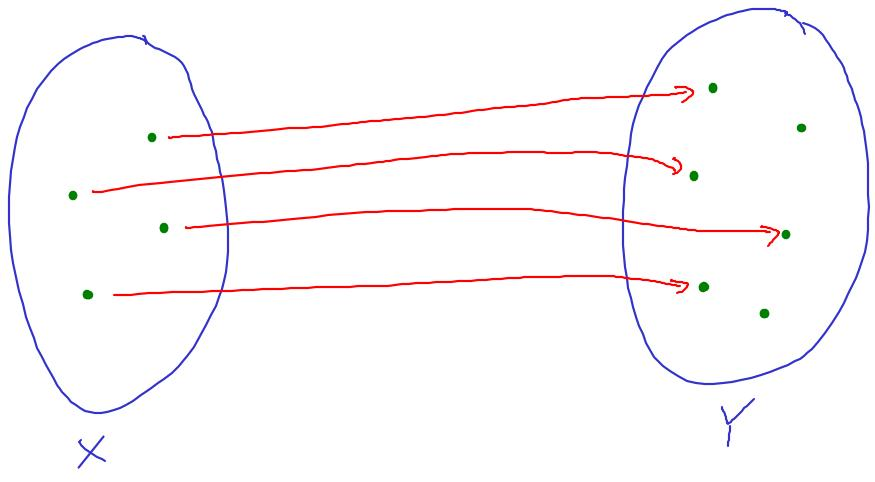
\includegraphics[width=7cm]{./_img/injsur4.jpeg}
        \centering \caption{injektiv, aber nicht surjektiv}
    \end{minipage}
    \quad
    \begin{minipage}{.48\textwidth}
        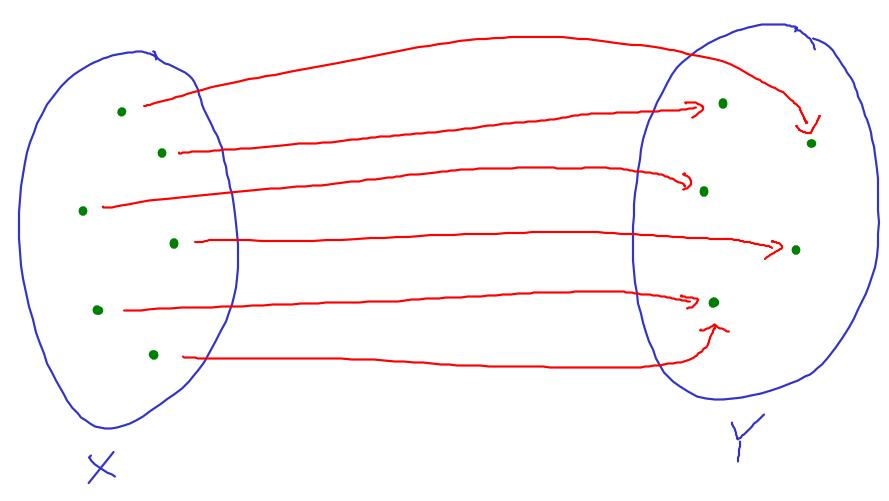
\includegraphics[width=7cm]{./_img/injsur2.jpeg}
        \centering \caption{surjektiv, aber nicht injektiv}
    \end{minipage}
    \quad\\[1em]
    \begin{minipage}{.48\textwidth}
        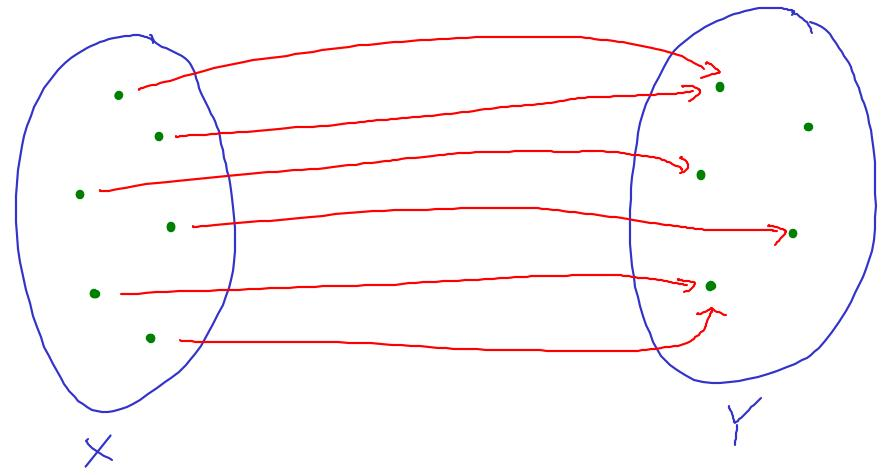
\includegraphics[width=7cm]{./_img/injsur1.jpeg}
        \centering \caption{weder injektiv noch surjektiv}
    \end{minipage}
    \quad
    \begin{minipage}{.48\textwidth}
        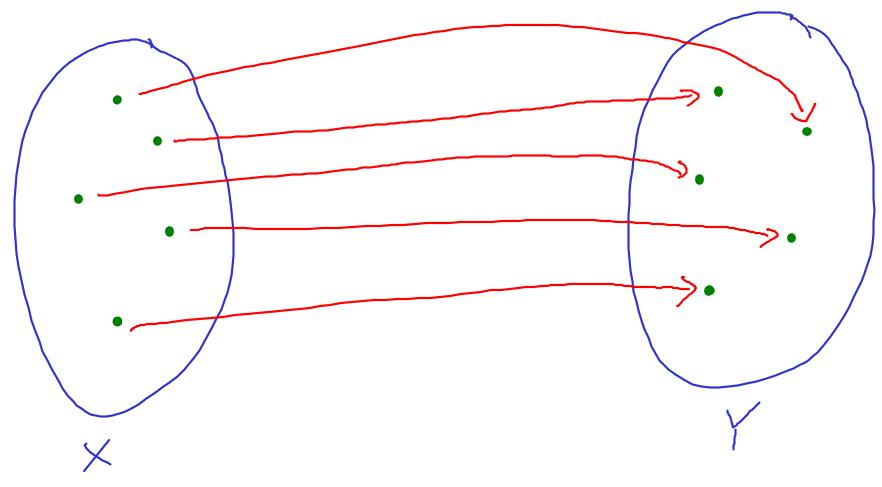
\includegraphics[width=7cm]{./_img/injsur3.jpeg}
        \centering \caption{bijektiv}
    \end{minipage}
\end{figure}


\begin{bsp} \label{bsp:injsur}
    Die vier Abbildungen
    \begin{align*}
        f_1 : \R \to \R \ &,\ x\mapsto x^2 & f_3 :\R\to \R_{\ge 0} \ &,\ x\mapsto x^2 \\
        f_2 : \R_{\ge 0} \to \R \ &,\ x\mapsto x^2 & f_4 :\R_{\ge 0} \to \R_{\ge 0} \ &,\ x\mapsto x^2
    \end{align*}
    sind, obwohl sie dieselbe Zuordnungsvorschrift haben, alle voneinander verschieden, weil sie verschiedene Definitions- oder Wertebereiche haben. Es gilt:
    \begin{enumerate}
        \item $f_1$ ist weder injektiv (wegen $f_1(1)=f_1(-1)$) noch surjektiv (wegen $-1\notin \im(f)$).
        \item $f_2$ ist injektiv (da jede reelle Zahl höchstens eines nichtnegative Quadratwurzel besitzt), aber nicht surjektiv.
        \item $f_3$ ist surjektiv (da jede nichtnegative reelle Zahl eine reelle Quadratwurzel besitzt), aber nicht injektiv.
        \item $f_4$ ist bijektiv. Denn jede nichtnegative reelle Zahl besitzt \emph{genau eine} nichtnegative reelle Quadratwurzel.
    \end{enumerate}
\end{bsp}


\begin{vorschau}[Abbildungen künstlich surjektiv machen] \label{surjektivmachen}
    Seien $X,Y$ zwei Mengen und $f:X\to Y$ eine Abbildung. Gemäß \cref{def:zielschrank} lässt sich der Wertebereich von $f$ auf die Menge $\im(f)$ einschränken. Die dadurch erhaltene Abbildung
        \[ f\vert^{\im(f)} : X \to \im(f) \ ,\ x\mapsto f(x) \]
    ist automatisch surjektiv, da es ja für jedes $y\in \im(f)$ mindestens ein $x\in X$ mit $f(x)=y$ gibt.

    Auf diese Weise ist es uns gelungen, $f$ „künstlich surjektiv“ zu machen. Ist uns daran gelegen, mit surjektiven Abbildungen zu arbeiten, so stellt das also kein Problem dar, da wir den Wertebereich einer Abbildung stets auf ihr Bild einschränken können.

    Ebenso ist es möglich, die Abbildung $f$ „künstlich injektiv“ zu machen. Dabei besteht der Trick darin, zwischen solchen Elementen von $X$, die unter $f$ denselben Funktionswert haben, „nicht mehr zu unterscheiden“. Die Technik „ähnliche Elemente nicht mehr voneinander zu unterscheiden“ wird in der LA1 eine prominente Rolle im Umfeld des sogenannten \href{https://de.wikipedia.org/wiki/Homomorphiesatz}{Homomorphiesatzes} spielen und kann mithilfe von \emph{Äquivalenzrelationen}, die im Relationenkapitel thematisiert werden, formalisiert werden, siehe \cref{teilmengenvsfaktormengen}.
\end{vorschau}





\section{Invertierbare Abbildungen}


In diesem Abschnitt seien stets $X,Y$ zwei Mengen und $f:X\to Y$ eine Abbildung.


\begin{defin}[Umkehrabbildung] \label{def:umkehrabb} \index{Umkehrabbildung} \index{Inverse Funktion} \index{invertierbare Abbildung} \index{Retraktion}
    Eine Abbildung $g:Y \to X$ heißt 
    \begin{itemize}
        \item \textbf{linksinvers zu $f$} (oder auch: eine \textbf{Retraktion von $f$}), falls $g\circ f=\id_X$.
        \item \textbf{rechtsinvers zu $f$}, falls $f\circ g=\id_Y$.
        \item \textbf{invers zu $f$} (oder auch: eine \textbf{Umkehrabbildung von $f$} oder eine \textbf{Inverse zu $f$}), falls sie sowohl links- als auch rechtsinvers zu $f$ ist.
    \end{itemize}
    $f$ heißt eine \textbf{invertierbare Abbildung}, wenn sie eine Umkehrabbildung besitzt.
\end{defin}


\begin{bsp} \label{bsp:umkehrabb} \qquad
    \begin{enumerate}
        \item Für jedes $k\in \N_0$ betrachte die beiden Abbildungen
        \begin{align*}
            f:\N_0 \to \N_0 \ &,\ n \mapsto n+1 \\
            g_k: \N_0 \to \N_0\ &,\ n \mapsto \begin{cases}
                n-1 & n\ge 1 \\
                k & n=0
            \end{cases}
        \end{align*}
        Dann gilt
        \begin{align*}
            (g_k\circ f)(n)&=g_k(n+1)=n && n\in \N_0 \\
            (f\circ g_k)(0) & = f(k) = k+1 \neq 0
        \end{align*}
        sodass $g_k\circ f=\id_{\N_0}$ aber $f\circ g_k\neq \id_{\N_0}$. Also ist zwar $g_k$ linksinvers zu $f$ (und dementsprechend $f$ rechtsinvers zu $g_k$), aber nicht rechtsinvers zu $f$.
        \[\begin{tikzcd}
            f\vcentcolon & 0 \ar[r, bend left]& 1 \ar[r, bend left]& 2 \ar[r, bend left]& 3 \ar[r, bend left]& 4 \ar[r, bend left]& 5 \ar[r, bend left]& \dots \\
            g_0\vcentcolon & 0 \ar[loop, out=145, in=215, looseness=5] & 1 \ar[l, bend right] & 2 \ar[l, bend right] & 3 \ar[l, bend right] & 4  \ar[l, bend right] & 5  \ar[l, bend right] &  \ar[l, bend right]  \dots
        \end{tikzcd}\]
        Von weiteren Abbildungen dieser Art handelt die Geschichte vom \href{https://en.wikipedia.org/wiki/Hilbert\%27s_paradox_of_the_Grand_Hotel}{Hilbert-Hotel}. Das Phänomen zweier Selbstabbildungen mit $g\circ f=\id$ aber $f\circ g\neq \id$ kann lediglich in unendlichen Mengen auftreten. Dedekind\footnote{\href{https://de.wikipedia.org/wiki/Richard_Dedekind}{Richard Dedekind (1831-1916)}} erhob eine ähnliche Aussage sogar zur Definition von Unendlichkeit: Eine Menge $X$ heißt \emph{Dedekind-unendlich}, wenn es eine injektive Abbildung $X\to X$ gibt, die nicht surjektiv ist.
        \item Die Abbildung
            \[ \Z\to \Z \ ,\ n\mapsto n+1 \]
        ist invertierbar, eine Inverse ist gegeben durch die Abbildung $n\mapsto n-1$.
        \item Die „Spiegelung an der $x$-Achse“
        \[ \R^2 \to \R^2 \ ,\ (x,y) \mapsto (x,-y) \]
        ist zu sich selbst invers.
        \item Sei $X$ eine beliebige Menge. Aus \cref{idneutral} folgt $\id_X\circ \id_X=\id_X$, sodass $\id_X$ eine invertierbare Abbildung ist, die invers zu sich selbst ist.\footnote{vgl. \cref{regelnfuerinv}a)}
    \end{enumerate}
\end{bsp}


\begin{satz}[Eindeutigkeit der Inversen]\label{umkehreind}
    Wenn $f$ eine invertierbare Abbildung ist, so gibt es auch nur \emph{genau eine} Umkehrabbildung zu $f$.\footnote{vgl. \cref{inveind}}
\end{satz}


\begin{bew}
    Seien $g,h:Y\to X$ zwei inverse Abbildungen zu $f$. Dann gilt:
    \begin{align*}
        g & = g\circ \id_Y && (\text{nach \cref{idneutral}})\\
        & = g\circ (f\circ h) && (\text{da $h$ invers zu $f$ ist}) \\
        & = (g\circ f)\circ h && (\text{nach \cref{abbassoziativ}}) \\
        & = \id_X \circ h && (\text{da $g$ invers zu $f$ ist}) \\
        & = h && (\text{nach \cref{idneutral}}) 
    \end{align*}
    Also ist die Inverse von $f$ eindeutig bestimmt. \qed
\end{bew}


\begin{bem}[\textbf{Die} Umkehrabbildung] \label{dieumkehrabb}
    Dieser Eindeutigkeitssatz berechtigt uns dazu, anstelle von „einer Umkehrabbildung von $f$“ von \emph{der} Umkehrabbildung von $f$ zu sprechen. 
    
    Die inverse Abbildung zu $f$ wird notiert mit
        \[ f^{-1} \]
    Beachte nochmal, dass es nur nur dann Sinn ergibt, von der „Umkehrabbildung $f^{-1}$“ zu sprechen, wenn $f$ invertierbar ist. Im Allgemeinen sind Abbildungen nicht invertierbar und wir werden mit \cref{invwiderleg} Techniken herleiten, mit denen sich dies beweisen lässt.
\end{bem}


\begin{bem}
    Das Zeichen „$f^{-1}$“ ist bereits in \cref{def:bildmenge} aufgetaucht und bezeichnete dort Fasern und Urbildmengen. Ist $f$ invertierbar, so trägt es also drei verschiedene Bedeutungen zugleich. Hier ist eine Tabelle mit den verschiedenen Bedeutungen von „$f$“ und „$f^{-1}$“:
    \[\begin{tabular}{cl}
        Zeichen & Bedeutung \\
        \midrule
        $f$ & Die Abbildung $X \to Y \ ,\ x \mapsto f(x)$ \\
        $f$ & Die (mengenwertige) Abbildung $\calP(X) \to \calP(Y) \ ,\ A\mapsto f(A)$  \\
        $f^{-1}$ & Die (mengenwertige) Abbildung $\calP(Y) \to \calP(X) \ ,\ B\mapsto f^{-1}(B)$ \\
        $f^{-1}$ & Die (mengenwertige) Abbildung $Y \to \calP(X) \ ,\ y\mapsto f^{-1}(y)$ \\
        \midrule
        $f^{-1}$ & Die Umkehrabbildung $f^{-1} : Y\to X \ ,\ y \mapsto f^{-1}(y)$ \\
        & (existiert nur, sofern $f$ invertierbar ist) 
    \end{tabular}\]
    Beachte, dass die ersten vier Ausdrücke immer Sinn ergeben; der fünfte aber nur dann, wenn $f$ invertierbar ist.
\end{bem}


\begin{bem}
    Nach \cref{umkehreind} ist die Inverse einer invertierbaren Abbildung stets eindeutig bestimmt. Eine bloße Links- oder Rechtsinverse braucht dagegen nicht eindeutig sein, wie \cref{bsp:umkehrabb}(1) zeigt.
\end{bem}


\begin{satz} \label{bijektiviso}
    Seien $X,Y$ zwei Mengen und $X\xrightarrow{f} Y$ eine Abbildung. Dann sind äquivalent:
    \begin{enumerate}[(i)]
        \item $f$ ist invertierbar.
        \item $f$ ist bijektiv.
    \end{enumerate}
\end{satz}


\begin{bew}\quad
    \begin{enumerate}
        \item[(ii)$\Rightarrow$(i):] Sei $f$ bijektiv. Dann gibt es für jedes $y\in Y$ genau ein $x\in X$ mit $f(x)=y$, sodass durch
            \[ g : Y\to X \ ,\ y \mapsto (\text{Das eindeutig bestimmte $x\in X$ mit $f(x)=y$}) \]
        eine Abbildung definiert ist. $g$ ist invers zu $f$, denn:
        \begin{enumerate}
            \item[($g\circ f=\id_X$):] Für ein beliebiges $a\in X$ ist
            \begin{align*}
                (g\circ f)(a) & = g(f(a)) \\
                & = (\text{Das eindeutig bestimmte $x\in X$ mit $f(x)=f(a)$}) \\
                & = a
            \end{align*}
            Weil $a\in X$ beliebig war, folgt die Gleichheit von Abbildungen $g\circ f=\id_X$.
            \item[($f\circ g=\id_Y$):] Für ein beliebiges $b\in Y$ ist
            \begin{align*}
                (f\circ g)(b) & = f(\text{Das eindeutig bestimmte $x\in X$ mit $f(x)=b$}) \\
                & = b
            \end{align*}
            Also ist $f\circ g=\id_Y$. 
        \end{enumerate}
        Insgesamt ist damit gezeigt, dass $g$ invers zu $f$ ist.
        \item[(i)$\Rightarrow$(ii):] Die Implikation (i)$\Rightarrow$(ii) ist Inhalt von \cref{aufg:bijektiviso}.\qed
    \end{enumerate}
\end{bew}


\begin{bsp} \quad
    \begin{enumerate}
        \item Nach \cref{bsp:injsur} ist die Abbildung
            \[ \R_{\ge 0} \to \R_{\ge 0} \ ,\ x \mapsto x^2 \]
        bijektiv. Ihre Inverse wird mit „$\sqrt{-}$” notiert. Für $y\in \R_{\ge 0}$ ist also „$\sqrt{y}$“ die eindeutig bestimmte nichtnegative reelle Zahl, die die Gleichung $(\sqrt{y})^2=y$ erfüllt. Ebenso gilt auch $\sqrt{x^2}=x$ für alle $x\in \R_{>0}$ (sogar schon für alle $x\in \R$).
        \item Subtraktion, Division, Wurzel und Logarithmus sind jeweils invers zu Addition, Multiplikation und Potenz:\begin{longtable}{clll}
            \phantom{Mengen} & Zuordnung: & ihre Inverse: & \phantom{Platzhalter}\\
            \midrule
            $\R\to \R$ & $x\mapsto x+a$ & $x\mapsto x-a$ & (für $a\in \R$)\\
            $\R\to \R$ & $x\mapsto ax$ & $x\mapsto \frac{x}{a}$ & (für $a\in \R\setminus \{0\}$) \\
            $\R_{> 0} \to \R_{> 0}$ & $x\mapsto x^a$ & $x\mapsto \sqrt[a]{x}$ & (für $a\in \R\setminus \{0\}$) \\
            $\R_{>0} \to \R_{>0}$ & $x \mapsto a^x$ & $x \mapsto \log_a(x)$ & (für $a\in \R_{>0}$)
        \end{longtable}
        Du bist es ja aus der Schule gewohnt, Gleichungen, die Summen, Produkte und Potenzen enthalten, aufzulösen mittels Subtrahieren, Dividieren, Wurzelziehen und Logarithmieren.
    \end{enumerate}
\end{bsp}


\begin{bem}[Bijektivität beweisen]
    Ist $f$ eine Abbildung, für die du beweisen möchtest, dass sie bjektiv ist, so stehen dir nun zwei Wege offen:
    \begin{enumerate}
        \item Du arbeitest mit \cref{def:bijektiv}, d.h. du beweist sowohl, dass $f$ injektiv ist, als auch, dass $f$ surjektiv ist.
        \item Du arbeitest mit \cref{bijektiviso}, d.h. du schreibst einen Kandidaten für die Umkehrabbildung hin und beweist daraufhin, dass er tatsächlich invers zu $f$ ist.
    \end{enumerate}
    Es gibt Situationen, in denen es schwer bis unmöglich ist, eine konkrete Abbildungsvorschrift für eine Umkehrabbildung anzugeben. In diesem Fall ist der erste Weg leichter.
    
    Es gibt aber auch Situationen wie z.B. in \cref{bsp:umkehrabb}(2), in denen du bei genauem „Hinsehen“ bereits einen Kandidaten für eine Umkehrabbildung ausfindig machen kannst. In diesem Fall bietet sich der zweite Weg an. Beachte auch, dass ein Beweis über den zweiten Weg stets informativer ist, da er dem Leser bereits die Gestalt der inversen Abbildung mitteilt.
\end{bem}


\begin{bem}[Invertierbarkeit widerlegen] \label{invwiderleg}
    Möchtest du beweisen, dass eine Abbildung keine Umkehrabbildung besitzt, so genügt es nach \cref{bijektiviso} bereits, wenn du beweist, dass sie nicht injektiv oder nicht surjektiv ist.
\end{bem}


\begin{bsp}
    Beispielsweise gilt:
    \begin{enumerate}
        \item Die Abbildung
            \[ f : \R \to \R \ ,\ x\mapsto x^2\]
        ist nicht invertierbar, weil sie nicht injektiv ist. Denn es ist zum Beispiel $f(-2)=f(2)$.
        \item Die Abbildung
            \[ f : \N_0 \to \N_0 \ ,\ n \mapsto n+1 \]
        ist nicht invertierbar, weil sie nicht surjektiv ist. Denn es ist $0\notin \im(f)$.
    \end{enumerate}
\end{bsp}





\clearpage
\section{Aufgabenvorschläge}


\begin{aufg}[Zerlegen von Abbildungen]
    Realisiert die folgenden Abbildungen als Verkettung möglichst elementarer Bausteine:
    \begin{enumerate}
        \item $\R\to \R \ ,\ x\mapsto (3x+1)^3$
        \item Sei $A$ die Menge aller Leute im Tutorium. Betrachte die Abbildung $f:A\to \N \ ,\ a\mapsto$ (die Anzahl der Wörter im Erstlingswerk des Literaturnobelpreisträgers im Geburtsjahr von $a$).
        \item $\calP(\R) \to \calP(\Q) \ ,\ X \mapsto \Q \setminus (X^c\cap \Z)$
        %\item $\N \to \N \ ,\ n \mapsto 3^n + n$\quad(schwierig)
    \end{enumerate}
\end{aufg}


\begin{aufg}[Wohldefiniertheit] \label{aufg:wohldef}
    An der Tafel von Captain Chaos stehen die folgenden Ausdrücke:
    \begin{align*}
        & (i) & \N \to \N\ &,\ n \mapsto n-1 \\[0.5em]
        & (ii) & \R\times \R \to \R \ &,\ (x,y) \mapsto \frac{x}{y} \\[0.5em]
        & (iii) & \Q \to \Z \ &,\ \frac{p}{q} \mapsto p-q \\[0.5em]
        & (iv) & \R \times \R \to \R \ &,\ (x,y) \mapsto x^y \\[0.5em]
        & (v) & \R \to \R \ &,\ x \mapsto \begin{cases}
            x^2+1\ , & \text{falls}\ x \le 0 \\
            x^2-1\ , & \text{falls}\ x\ge 0
        \end{cases}
    \end{align*}
    Was haltet ihr davon?
\end{aufg}


\begin{aufg}[injektiv, surjektiv, bijektiv]
    Untersucht die folgenden Abbildungen darauf, ob sie injektiv, surjektiv oder bijektiv sind:
    \begin{align*}
        & \text{a)} & \R \to \R\ &,\ x\mapsto 3x+1 \\
        & \text{b)} & \Z \to \Z\ &,\ n\mapsto 2n \\
        & \text{c)} & \Z \times \N_{\ge 1} \to \Q\ &,\ (z,n) \mapsto \frac{z}{n} \\
        & \text{d)} & X\xrightarrow{\id} X\ & && (\text{für eine beliebige Menge $X$}) \\
        & \text{e)} & \calP(\R) \to \calP(\R) \ &,\ A \mapsto A^c
    \end{align*}
\end{aufg}


\begin{aufg}[Vererbung von Injektivität und Surjektivität] \label{aufg:bijektiviso}
    Seien $X,Y,Z$ drei beliebige Mengen und $X \xrightarrow{f} Y \xrightarrow{g} Z$ zwei Abbildungen. Beweist die folgenden Implikationen:
    \begin{enumerate}
        \item $f,g$ injektiv $\implies$ $g\circ f$ injektiv $\implies$ $f$ injektiv.
        \item $f,g$ surjektiv $\implies$ $g\circ f$ surjektiv $\implies$ $g$ surjektiv.
        \item Invertierbare Abbildungen sind bijektiv.
    \end{enumerate}
    Könnt ihr euch a) und b) im Beweis von c) zunutze machen?
\end{aufg}

